\documentclass[a4paper,11pt]{article}
\usepackage{ctex}

\setCJKmainfont{FandolSong-Regular}
\setCJKsansfont{FandolSong-Bold}
\setCJKfamilyfont{italic}{FandolKai-Regular}
\newcommand{\CJKtextit}[1]{{\CJKfamily{italic}#1}}

\usepackage[breakable]{tcolorbox}
\usepackage{parskip} % Stop auto-indenting (to mimic markdown behaviour)

% Basic figure setup, for now with no caption control since it's done
% automatically by Pandoc (which extracts ![](path) syntax from Markdown).
\usepackage{graphicx}
% Maintain compatibility with old templates. Remove in nbconvert 6.0
% \let\Oldincludegraphics\includegraphics
% Ensure that by default, figures have no caption (until we provide a
% proper Figure object with a Caption API and a way to capture that
% in the conversion process - todo).
\usepackage{caption}
% \DeclareCaptionFormat{nocaption}{}
% \captionsetup{format=nocaption,aboveskip=0pt,belowskip=0pt}
\usepackage{float}
\floatplacement{figure}{H} % forces figures to be placed at the correct location
\usepackage{xcolor} % Allow colors to be defined
\usepackage{enumerate} % Needed for markdown enumerations to work
\usepackage{geometry} % Used to adjust the document margins
\usepackage{amsmath} % Equations
\usepackage{amssymb} % Equations
\usepackage{diagbox,multirow}
\usepackage{textcomp,tocloft} % defines textquotesingle
% Hack from http://tex.stackexchange.com/a/47451/13684:
\AtBeginDocument{%
    \def\PYZsq{\textquotesingle}% Upright quotes in Pygmentized code
}
\usepackage{upquote} % Upright quotes for verbatim code
\usepackage{eurosym} % defines \euro
\usepackage{iftex}
\ifPDFTeX
    \usepackage[T1]{fontenc}
    \IfFileExists{alphabeta.sty}{
          \usepackage{alphabeta}
      }{
          \usepackage[mathletters]{ucs}
          \usepackage[utf8x]{inputenc}
      }
\else
    \usepackage{fontspec}
    \usepackage{unicode-math}
\fi
\usepackage{fancyvrb} % verbatim replacement that allows latex
\usepackage{grffile} % extends the file name processing of package graphics
                     % to support a larger range
\makeatletter % fix for old versions of grffile with XeLaTeX
\@ifpackagelater{grffile}{2019/11/01}
{
  % Do nothing on new versions
}
{
  \def\Gread@@xetex#1{%
    \IfFileExists{"\Gin@base".bb}%
    {\Gread@eps{\Gin@base.bb}}%
    {\Gread@@xetex@aux#1}%
  }
}
\makeatother
\usepackage[Export]{adjustbox} % Used to constrain images to a maximum size
\adjustboxset{max size={1.0\linewidth}{1.0\paperheight}}
% The hyperref package gives us a pdf with properly built
% internal navigation ('pdf bookmarks' for the table of contents,
% internal cross-reference links, web links for URLs, etc.)
\usepackage{hyperref}
% The default LaTeX title has an obnoxious amount of whitespace. By default,
% titling removes some of it. It also provides customization options.
\usepackage{titling}
\usepackage{longtable} % longtable support required by pandoc >1.10
\usepackage{booktabs}  % table support for pandoc > 1.12.2
\usepackage{array}     % table support for pandoc >= 2.11.3
\usepackage{calc}      % table minipage width calculation for pandoc >= 2.11.1
\usepackage[inline]{enumitem} % IRkernel/repr support (it uses the enumerate* environment)
\usepackage[normalem]{ulem} % ulem is needed to support strikethroughs (\sout)
                            % normalem makes italics be italics, not underlines
\usepackage{soul}      % strikethrough (\st) support for pandoc >= 3.0.0
\usepackage{mathrsfs}
\usepackage{algorithm,algpseudocode,multirow}
\usepackage{lipsum}

\usepackage{fontawesome5}
\newcommand{\email}[1]{\faEnvelope\ {#1}}
\newfontfamily\symbolfont{Symbol}
\newcommand{\symbolpi}{\text{\symbolfont π}}

% Load FontAwesome symbols
%%%%%%%%%%%%%%%%%%%%%%%%%%%%%%%%%%%%%%%%%%%%%%%%%%%%%%%%        
%   Define new font families for Font Awesome symbols  %
%%%%%%%%%%%%%%%%%%%%%%%%%%%%%%%%%%%%%%%%%%%%%%%%%%%%%%%%  
\newfontfamily{\FABrands}
[Path = fontawesome/, 
Scale = 0.85, Extension = .otf]
{FontAwesome6Brands}

\newfontfamily{\FARegular}
[Path = fontawesome/, 
Scale = 0.85, Extension = .otf]
{FontAwesome6Regular}

\newfontfamily{\FASolid}
[Path = fontawesome/, 
Scale = 0.95, Extension = .otf]
{FontAwesome6Solid}

\newcommand{\faBrands}[1]{{\FABrands\symbol{"#1}}}
\newcommand{\faRegular}[1]{{\FARegular\symbol{"#1}}}
\newcommand{\faSolid}[1]{{\FASolid\symbol{"#1}}}

%%%%%%%%%%%%%%%%%%%%%%%%%%%%
%      Example usage       %
%%%%%%%%%%%%%%%%%%%%%%%%%%%%

\def\faEnvelope{\faSolid{F0E0}}
\def\faEnvelopeO{\faRegular{F0E0}}
\def\faPhone{\faSolid{F095}}
\def\faGithub{\faBrands{F09B}}
\def\faGoogleScholar{\faBrands{E63B}}
\def\faOrcid{\faBrands{F8D2}}
\def\faCrossHairs{\faSolid{F05B}}
\def\faBullseye{\faSolid{F140}}

\def\faHeartbeat{\faSolid{F21E}}
\def\faGraduationCap{\faSolid{F19D}}
\def\faUniversity{\faSolid{F19C}}
\def\faUsers{\faSolid{F0C0}}
\def\faProject{\faSolid{F542}}
\def\faSquare{\faSolid{F0C8}}
\def\faCogs{\faSolid{F085}}
\def\faCog{\faSolid{F013}}
\def\faMusic{\faSolid{F001}}
\def\faPlay{\faSolid{F04B}}
\def\faFile{\faRegular{F15C}}
\def\faBook{\faSolid{F02D}}

% Companies
\def\faMicrosoft{\faBrands{F3CA}}
\def\faApple{\faBrands{F179}}
\def\faGoogle{\faBrands{F1A0}}
\def\faMeta{\faBrands{E49B}}
\def\faFacebook{\faBrands{F09A}}
\def\faTwitter{\faBrands{F099}}
\def\faXTwitter{\faBrands{E61B}}


% Colors for the hyperref package
% \definecolor{urlcolor}{rgb}{0,.145,.698}
% \definecolor{linkcolor}{rgb}{.71,0.21,0.01}
% \definecolor{citecolor}{rgb}{.12,.54,.11}
% ANSI colors
\definecolor{ansi-black}{HTML}{3E424D}
\definecolor{ansi-black-intense}{HTML}{282C36}
\definecolor{ansi-red}{HTML}{E75C58}
\definecolor{ansi-red-intense}{HTML}{B22B31}
\definecolor{ansi-green}{HTML}{00A250}
\definecolor{ansi-green-intense}{HTML}{007427}
\definecolor{ansi-yellow}{HTML}{DDB62B}
\definecolor{ansi-yellow-intense}{HTML}{B27D12}
\definecolor{ansi-blue}{HTML}{208FFB}
\definecolor{ansi-blue-intense}{HTML}{0065CA}
\definecolor{ansi-magenta}{HTML}{D160C4}
\definecolor{ansi-magenta-intense}{HTML}{A03196}
\definecolor{ansi-cyan}{HTML}{60C6C8}
\definecolor{ansi-cyan-intense}{HTML}{258F8F}
\definecolor{ansi-white}{HTML}{C5C1B4}
\definecolor{ansi-white-intense}{HTML}{A1A6B2}
\definecolor{ansi-default-inverse-fg}{HTML}{FFFFFF}
\definecolor{ansi-default-inverse-bg}{HTML}{000000}
% common color for the border for error outputs.
\definecolor{outerrorbackground}{HTML}{FFDFDF}
% commands and environments needed by pandoc snippets
% extracted from the output of `pandoc -s`
\providecommand{\tightlist}{%
  \setlength{\itemsep}{0pt}\setlength{\parskip}{0pt}}
\DefineVerbatimEnvironment{Highlighting}{Verbatim}{commandchars=\\\{\}}
% Add ',fontsize=\small' for more characters per line
\newenvironment{Shaded}{}{}
\newcommand{\KeywordTok}[1]{\textcolor[rgb]{0.00,0.44,0.13}{\textbf{{#1}}}}
\newcommand{\DataTypeTok}[1]{\textcolor[rgb]{0.56,0.13,0.00}{{#1}}}
\newcommand{\DecValTok}[1]{\textcolor[rgb]{0.25,0.63,0.44}{{#1}}}
\newcommand{\BaseNTok}[1]{\textcolor[rgb]{0.25,0.63,0.44}{{#1}}}
\newcommand{\FloatTok}[1]{\textcolor[rgb]{0.25,0.63,0.44}{{#1}}}
\newcommand{\CharTok}[1]{\textcolor[rgb]{0.25,0.44,0.63}{{#1}}}
\newcommand{\StringTok}[1]{\textcolor[rgb]{0.25,0.44,0.63}{{#1}}}
\newcommand{\CommentTok}[1]{\textcolor[rgb]{0.38,0.63,0.69}{\textit{{#1}}}}
\newcommand{\OtherTok}[1]{\textcolor[rgb]{0.00,0.44,0.13}{{#1}}}
\newcommand{\AlertTok}[1]{\textcolor[rgb]{1.00,0.00,0.00}{\textbf{{#1}}}}
\newcommand{\FunctionTok}[1]{\textcolor[rgb]{0.02,0.16,0.49}{{#1}}}
\newcommand{\RegionMarkerTok}[1]{{#1}}
\newcommand{\ErrorTok}[1]{\textcolor[rgb]{1.00,0.00,0.00}{\textbf{{#1}}}}
\newcommand{\NormalTok}[1]{{#1}}
% Additional commands for more recent versions of Pandoc
\newcommand{\ConstantTok}[1]{\textcolor[rgb]{0.53,0.00,0.00}{{#1}}}
\newcommand{\SpecialCharTok}[1]{\textcolor[rgb]{0.25,0.44,0.63}{{#1}}}
\newcommand{\VerbatimStringTok}[1]{\textcolor[rgb]{0.25,0.44,0.63}{{#1}}}
\newcommand{\SpecialStringTok}[1]{\textcolor[rgb]{0.73,0.40,0.53}{{#1}}}
\newcommand{\ImportTok}[1]{{#1}}
\newcommand{\DocumentationTok}[1]{\textcolor[rgb]{0.73,0.13,0.13}{\textit{{#1}}}}
\newcommand{\AnnotationTok}[1]{\textcolor[rgb]{0.38,0.63,0.69}{\textbf{\textit{{#1}}}}}
\newcommand{\CommentVarTok}[1]{\textcolor[rgb]{0.38,0.63,0.69}{\textbf{\textit{{#1}}}}}
\newcommand{\VariableTok}[1]{\textcolor[rgb]{0.10,0.09,0.49}{{#1}}}
\newcommand{\ControlFlowTok}[1]{\textcolor[rgb]{0.00,0.44,0.13}{\textbf{{#1}}}}
\newcommand{\OperatorTok}[1]{\textcolor[rgb]{0.40,0.40,0.40}{{#1}}}
\newcommand{\BuiltInTok}[1]{{#1}}
\newcommand{\ExtensionTok}[1]{{#1}}
\newcommand{\PreprocessorTok}[1]{\textcolor[rgb]{0.74,0.48,0.00}{{#1}}}
\newcommand{\AttributeTok}[1]{\textcolor[rgb]{0.49,0.56,0.16}{{#1}}}
\newcommand{\InformationTok}[1]{\textcolor[rgb]{0.38,0.63,0.69}{\textbf{\textit{{#1}}}}}
\newcommand{\WarningTok}[1]{\textcolor[rgb]{0.38,0.63,0.69}{\textbf{\textit{{#1}}}}}
% Define a nice break command that doesn't care if a line doesn't already
% exist.
\def\br{\hspace*{\fill} \\* }
% Math Jax compatibility definitions
\def\gt{>}
\def\lt{<}
\let\Oldtex\TeX
\let\Oldlatex\LaTeX
\renewcommand{\TeX}{\textrm{\Oldtex}}
\renewcommand{\LaTeX}{\textrm{\Oldlatex}}
% Document parameters

% Document title
\title{\huge
\CJKtextit{n\&k光学量测设备的调研} \\
\vspace{0.5cm}
\rule{\linewidth}{0.1mm} \\
\vspace{2cm}
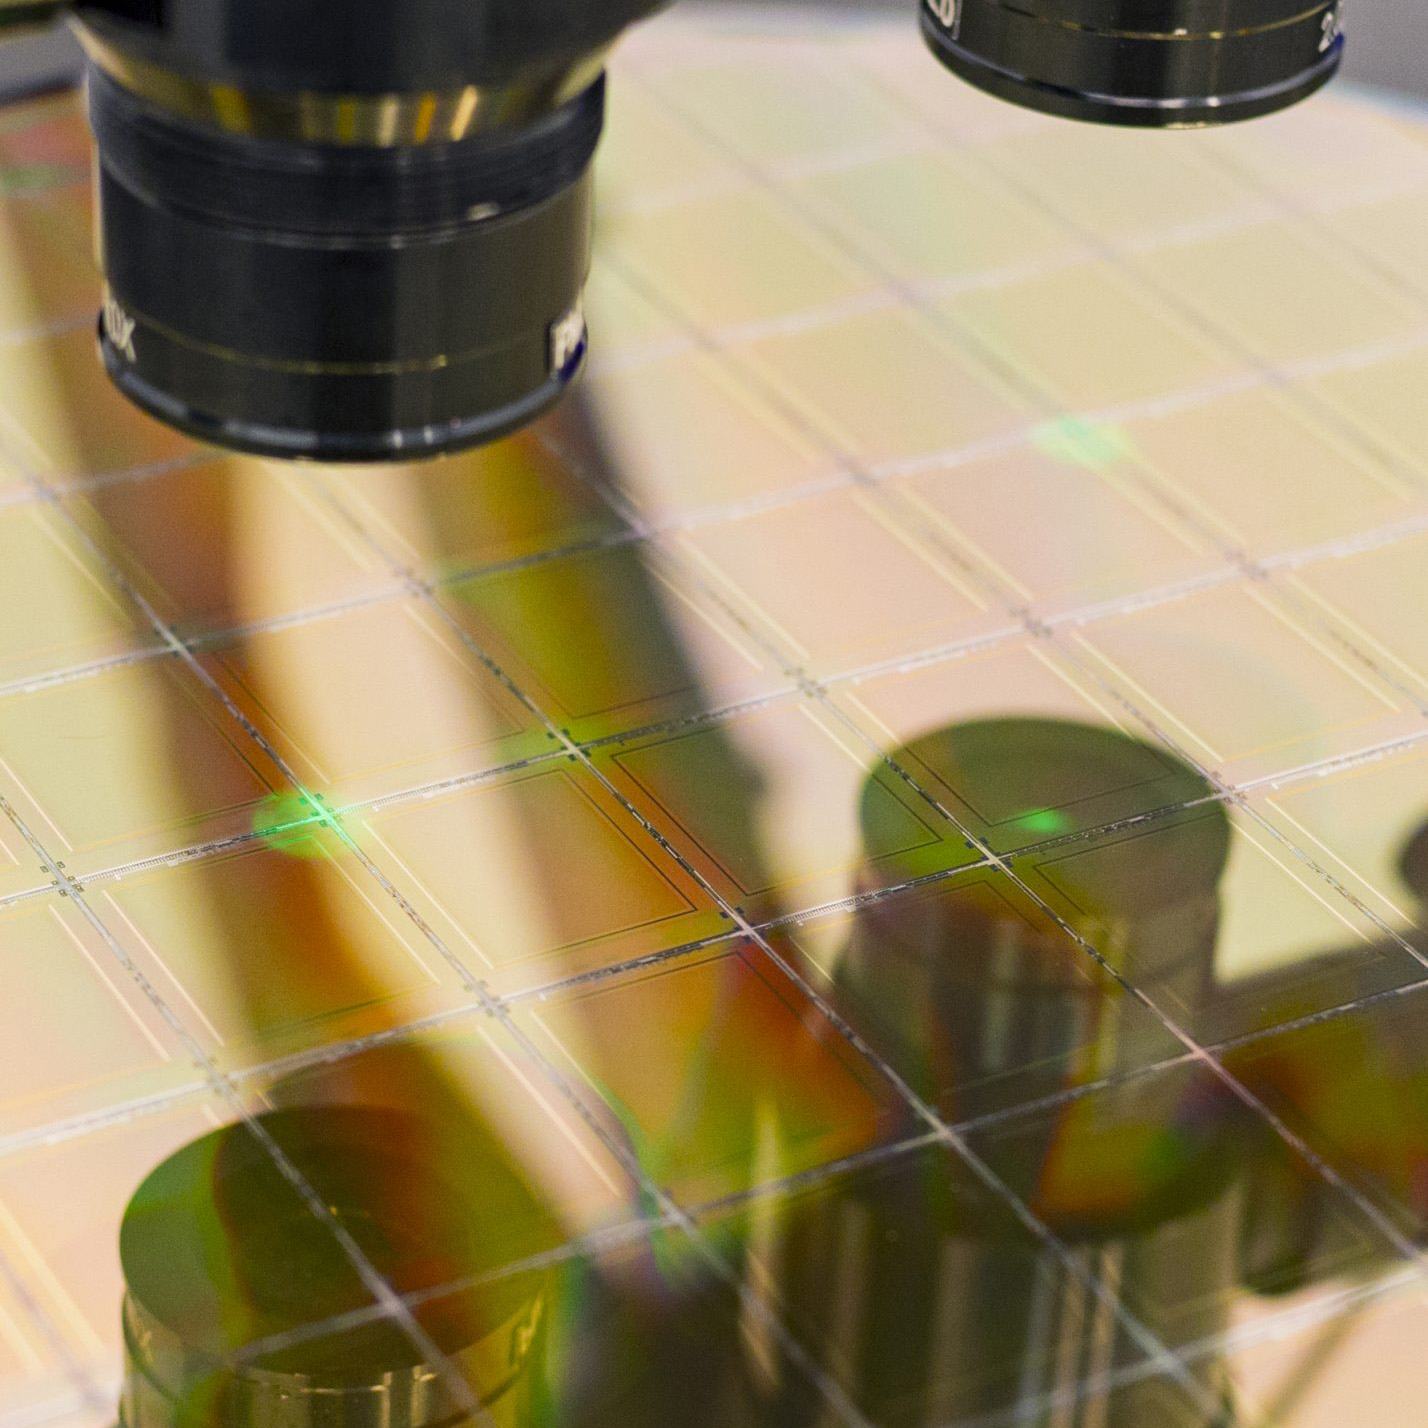
\includegraphics[scale=0.6]{nandk_deposit_photos.jpg} \\
\vspace{1.5cm}
\LARGE 功率器件量测机台 \\
$\mathtt{Olympian}~\&~\mathtt{OptiPrime(X)}$系列 \\
\vspace{1cm} 
\LARGE 陈昂\medskip}

\author{
\color{magenta}\email{\href{mailto:chenang@outlook.com}{\LARGE\texttt{chenang@outlook.com}}}\\
% \color{magenta}\email{\href{mailto:yj.ma@mzsemi.com}{\LARGE\texttt{yj.ma@mzsemi.com}}}\\
% \color{magenta}\email{\href{mailto:xy.shi@mzsime.com}{\LARGE\texttt{xy.shi@mzsime.com}}}\\
\medskip}
\date{\LARGE\today}
% \date{\LARGE 2025年5月15日}
    
% Pygments definitions
\makeatletter
\def\PY@reset{\let\PY@it=\relax \let\PY@bf=\relax%
    \let\PY@ul=\relax \let\PY@tc=\relax%
    \let\PY@bc=\relax \let\PY@ff=\relax}
\def\PY@tok#1{\csname PY@tok@#1\endcsname}
\def\PY@toks#1+{\ifx\relax#1\empty\else%
    \PY@tok{#1}\expandafter\PY@toks\fi}
\def\PY@do#1{\PY@bc{\PY@tc{\PY@ul{%
    \PY@it{\PY@bf{\PY@ff{#1}}}}}}}
\def\PY#1#2{\PY@reset\PY@toks#1+\relax+\PY@do{#2}}

\@namedef{PY@tok@w}{\def\PY@tc##1{\textcolor[rgb]{0.73,0.73,0.73}{##1}}}
\@namedef{PY@tok@c}{\let\PY@it=\textit\def\PY@tc##1{\textcolor[rgb]{0.24,0.48,0.48}{##1}}}
\@namedef{PY@tok@cp}{\def\PY@tc##1{\textcolor[rgb]{0.61,0.40,0.00}{##1}}}
\@namedef{PY@tok@k}{\let\PY@bf=\textbf\def\PY@tc##1{\textcolor[rgb]{0.00,0.50,0.00}{##1}}}
\@namedef{PY@tok@kp}{\def\PY@tc##1{\textcolor[rgb]{0.00,0.50,0.00}{##1}}}
\@namedef{PY@tok@kt}{\def\PY@tc##1{\textcolor[rgb]{0.69,0.00,0.25}{##1}}}
\@namedef{PY@tok@o}{\def\PY@tc##1{\textcolor[rgb]{0.40,0.40,0.40}{##1}}}
\@namedef{PY@tok@ow}{\let\PY@bf=\textbf\def\PY@tc##1{\textcolor[rgb]{0.67,0.13,1.00}{##1}}}
\@namedef{PY@tok@nb}{\def\PY@tc##1{\textcolor[rgb]{0.00,0.50,0.00}{##1}}}
\@namedef{PY@tok@nf}{\def\PY@tc##1{\textcolor[rgb]{0.00,0.00,1.00}{##1}}}
\@namedef{PY@tok@nc}{\let\PY@bf=\textbf\def\PY@tc##1{\textcolor[rgb]{0.00,0.00,1.00}{##1}}}
\@namedef{PY@tok@nn}{\let\PY@bf=\textbf\def\PY@tc##1{\textcolor[rgb]{0.00,0.00,1.00}{##1}}}
\@namedef{PY@tok@ne}{\let\PY@bf=\textbf\def\PY@tc##1{\textcolor[rgb]{0.80,0.25,0.22}{##1}}}
\@namedef{PY@tok@nv}{\def\PY@tc##1{\textcolor[rgb]{0.10,0.09,0.49}{##1}}}
\@namedef{PY@tok@no}{\def\PY@tc##1{\textcolor[rgb]{0.53,0.00,0.00}{##1}}}
\@namedef{PY@tok@nl}{\def\PY@tc##1{\textcolor[rgb]{0.46,0.46,0.00}{##1}}}
\@namedef{PY@tok@ni}{\let\PY@bf=\textbf\def\PY@tc##1{\textcolor[rgb]{0.44,0.44,0.44}{##1}}}
\@namedef{PY@tok@na}{\def\PY@tc##1{\textcolor[rgb]{0.41,0.47,0.13}{##1}}}
\@namedef{PY@tok@nt}{\let\PY@bf=\textbf\def\PY@tc##1{\textcolor[rgb]{0.00,0.50,0.00}{##1}}}
\@namedef{PY@tok@nd}{\def\PY@tc##1{\textcolor[rgb]{0.67,0.13,1.00}{##1}}}
\@namedef{PY@tok@s}{\def\PY@tc##1{\textcolor[rgb]{0.73,0.13,0.13}{##1}}}
\@namedef{PY@tok@sd}{\let\PY@it=\textit\def\PY@tc##1{\textcolor[rgb]{0.73,0.13,0.13}{##1}}}
\@namedef{PY@tok@si}{\let\PY@bf=\textbf\def\PY@tc##1{\textcolor[rgb]{0.64,0.35,0.47}{##1}}}
\@namedef{PY@tok@se}{\let\PY@bf=\textbf\def\PY@tc##1{\textcolor[rgb]{0.67,0.36,0.12}{##1}}}
\@namedef{PY@tok@sr}{\def\PY@tc##1{\textcolor[rgb]{0.64,0.35,0.47}{##1}}}
\@namedef{PY@tok@ss}{\def\PY@tc##1{\textcolor[rgb]{0.10,0.09,0.49}{##1}}}
\@namedef{PY@tok@sx}{\def\PY@tc##1{\textcolor[rgb]{0.00,0.50,0.00}{##1}}}
\@namedef{PY@tok@m}{\def\PY@tc##1{\textcolor[rgb]{0.40,0.40,0.40}{##1}}}
\@namedef{PY@tok@gh}{\let\PY@bf=\textbf\def\PY@tc##1{\textcolor[rgb]{0.00,0.00,0.50}{##1}}}
\@namedef{PY@tok@gu}{\let\PY@bf=\textbf\def\PY@tc##1{\textcolor[rgb]{0.50,0.00,0.50}{##1}}}
\@namedef{PY@tok@gd}{\def\PY@tc##1{\textcolor[rgb]{0.63,0.00,0.00}{##1}}}
\@namedef{PY@tok@gi}{\def\PY@tc##1{\textcolor[rgb]{0.00,0.52,0.00}{##1}}}
\@namedef{PY@tok@gr}{\def\PY@tc##1{\textcolor[rgb]{0.89,0.00,0.00}{##1}}}
\@namedef{PY@tok@ge}{\let\PY@it=\textit}
\@namedef{PY@tok@gs}{\let\PY@bf=\textbf}
\@namedef{PY@tok@ges}{\let\PY@bf=\textbf\let\PY@it=\textit}
\@namedef{PY@tok@gp}{\let\PY@bf=\textbf\def\PY@tc##1{\textcolor[rgb]{0.00,0.00,0.50}{##1}}}
\@namedef{PY@tok@go}{\def\PY@tc##1{\textcolor[rgb]{0.44,0.44,0.44}{##1}}}
\@namedef{PY@tok@gt}{\def\PY@tc##1{\textcolor[rgb]{0.00,0.27,0.87}{##1}}}
\@namedef{PY@tok@err}{\def\PY@bc##1{{\setlength{\fboxsep}{\string -\fboxrule}\fcolorbox[rgb]{1.00,0.00,0.00}{1,1,1}{\strut ##1}}}}
\@namedef{PY@tok@kc}{\let\PY@bf=\textbf\def\PY@tc##1{\textcolor[rgb]{0.00,0.50,0.00}{##1}}}
\@namedef{PY@tok@kd}{\let\PY@bf=\textbf\def\PY@tc##1{\textcolor[rgb]{0.00,0.50,0.00}{##1}}}
\@namedef{PY@tok@kn}{\let\PY@bf=\textbf\def\PY@tc##1{\textcolor[rgb]{0.00,0.50,0.00}{##1}}}
\@namedef{PY@tok@kr}{\let\PY@bf=\textbf\def\PY@tc##1{\textcolor[rgb]{0.00,0.50,0.00}{##1}}}
\@namedef{PY@tok@bp}{\def\PY@tc##1{\textcolor[rgb]{0.00,0.50,0.00}{##1}}}
\@namedef{PY@tok@fm}{\def\PY@tc##1{\textcolor[rgb]{0.00,0.00,1.00}{##1}}}
\@namedef{PY@tok@vc}{\def\PY@tc##1{\textcolor[rgb]{0.10,0.09,0.49}{##1}}}
\@namedef{PY@tok@vg}{\def\PY@tc##1{\textcolor[rgb]{0.10,0.09,0.49}{##1}}}
\@namedef{PY@tok@vi}{\def\PY@tc##1{\textcolor[rgb]{0.10,0.09,0.49}{##1}}}
\@namedef{PY@tok@vm}{\def\PY@tc##1{\textcolor[rgb]{0.10,0.09,0.49}{##1}}}
\@namedef{PY@tok@sa}{\def\PY@tc##1{\textcolor[rgb]{0.73,0.13,0.13}{##1}}}
\@namedef{PY@tok@sb}{\def\PY@tc##1{\textcolor[rgb]{0.73,0.13,0.13}{##1}}}
\@namedef{PY@tok@sc}{\def\PY@tc##1{\textcolor[rgb]{0.73,0.13,0.13}{##1}}}
\@namedef{PY@tok@dl}{\def\PY@tc##1{\textcolor[rgb]{0.73,0.13,0.13}{##1}}}
\@namedef{PY@tok@s2}{\def\PY@tc##1{\textcolor[rgb]{0.73,0.13,0.13}{##1}}}
\@namedef{PY@tok@sh}{\def\PY@tc##1{\textcolor[rgb]{0.73,0.13,0.13}{##1}}}
\@namedef{PY@tok@s1}{\def\PY@tc##1{\textcolor[rgb]{0.73,0.13,0.13}{##1}}}
\@namedef{PY@tok@mb}{\def\PY@tc##1{\textcolor[rgb]{0.40,0.40,0.40}{##1}}}
\@namedef{PY@tok@mf}{\def\PY@tc##1{\textcolor[rgb]{0.40,0.40,0.40}{##1}}}
\@namedef{PY@tok@mh}{\def\PY@tc##1{\textcolor[rgb]{0.40,0.40,0.40}{##1}}}
\@namedef{PY@tok@mi}{\def\PY@tc##1{\textcolor[rgb]{0.40,0.40,0.40}{##1}}}
\@namedef{PY@tok@il}{\def\PY@tc##1{\textcolor[rgb]{0.40,0.40,0.40}{##1}}}
\@namedef{PY@tok@mo}{\def\PY@tc##1{\textcolor[rgb]{0.40,0.40,0.40}{##1}}}
\@namedef{PY@tok@ch}{\let\PY@it=\textit\def\PY@tc##1{\textcolor[rgb]{0.24,0.48,0.48}{##1}}}
\@namedef{PY@tok@cm}{\let\PY@it=\textit\def\PY@tc##1{\textcolor[rgb]{0.24,0.48,0.48}{##1}}}
\@namedef{PY@tok@cpf}{\let\PY@it=\textit\def\PY@tc##1{\textcolor[rgb]{0.24,0.48,0.48}{##1}}}
\@namedef{PY@tok@c1}{\let\PY@it=\textit\def\PY@tc##1{\textcolor[rgb]{0.24,0.48,0.48}{##1}}}
\@namedef{PY@tok@cs}{\let\PY@it=\textit\def\PY@tc##1{\textcolor[rgb]{0.24,0.48,0.48}{##1}}}

\def\PYZbs{\char`\\}
\def\PYZus{\char`\_}
\def\PYZob{\char`\{}
\def\PYZcb{\char`\}}
\def\PYZca{\char`\^}
\def\PYZam{\char`\&}
\def\PYZlt{\char`\<}
\def\PYZgt{\char`\>}
\def\PYZsh{\char`\#}
\def\PYZpc{\char`\%}
\def\PYZdl{\char`\$}
\def\PYZhy{\char`\-}
\def\PYZsq{\char`\'}
\def\PYZdq{\char`\"}
\def\PYZti{\char`\~}
% for compatibility with earlier versions
\def\PYZat{@}
\def\PYZlb{[}
\def\PYZrb{]}
\makeatother


% For linebreaks inside Verbatim environment from package fancyvrb.
\makeatletter
\newbox\Wrappedcontinuationbox
\newbox\Wrappedvisiblespacebox
\newcommand*\Wrappedvisiblespace {\textcolor{red}{\textvisiblespace}}
\newcommand*\Wrappedcontinuationsymbol {\textcolor{red}{\llap{\tiny$\m@th\hookrightarrow$}}}
\newcommand*\Wrappedcontinuationindent {3ex }
\newcommand*\Wrappedafterbreak {\kern\Wrappedcontinuationindent\copy\Wrappedcontinuationbox}
% Take advantage of the already applied Pygments mark-up to insert
% potential linebreaks for TeX processing.
%        {, <, #, %, $, ' and ": go to next line.
%        _, }, ^, &, >, - and ~: stay at end of broken line.
% Use of \textquotesingle for straight quote.
\newcommand*\Wrappedbreaksatspecials {%
    \def\PYGZus{\discretionary{\char`\_}{\Wrappedafterbreak}{\char`\_}}%
    \def\PYGZob{\discretionary{}{\Wrappedafterbreak\char`\{}{\char`\{}}%
    \def\PYGZcb{\discretionary{\char`\}}{\Wrappedafterbreak}{\char`\}}}%
    \def\PYGZca{\discretionary{\char`\^}{\Wrappedafterbreak}{\char`\^}}%
    \def\PYGZam{\discretionary{\char`\&}{\Wrappedafterbreak}{\char`\&}}%
    \def\PYGZlt{\discretionary{}{\Wrappedafterbreak\char`\<}{\char`\<}}%
    \def\PYGZgt{\discretionary{\char`\>}{\Wrappedafterbreak}{\char`\>}}%
    \def\PYGZsh{\discretionary{}{\Wrappedafterbreak\char`\#}{\char`\#}}%
    \def\PYGZpc{\discretionary{}{\Wrappedafterbreak\char`\%}{\char`\%}}%
    \def\PYGZdl{\discretionary{}{\Wrappedafterbreak\char`\$}{\char`\$}}%
    \def\PYGZhy{\discretionary{\char`\-}{\Wrappedafterbreak}{\char`\-}}%
    \def\PYGZsq{\discretionary{}{\Wrappedafterbreak\textquotesingle}{\textquotesingle}}%
    \def\PYGZdq{\discretionary{}{\Wrappedafterbreak\char`\"}{\char`\"}}%
    \def\PYGZti{\discretionary{\char`\~}{\Wrappedafterbreak}{\char`\~}}%
}
% Some characters . , ; ? ! / are not pygmentized.
% This macro makes them "active" and they will insert potential linebreaks
\newcommand*\Wrappedbreaksatpunct {%
    \lccode`\~`\.\lowercase{\def~}{\discretionary{\hbox{\char`\.}}{\Wrappedafterbreak}{\hbox{\char`\.}}}%
    \lccode`\~`\,\lowercase{\def~}{\discretionary{\hbox{\char`\,}}{\Wrappedafterbreak}{\hbox{\char`\,}}}%
    \lccode`\~`\;\lowercase{\def~}{\discretionary{\hbox{\char`\;}}{\Wrappedafterbreak}{\hbox{\char`\;}}}%
    \lccode`\~`\:\lowercase{\def~}{\discretionary{\hbox{\char`\:}}{\Wrappedafterbreak}{\hbox{\char`\:}}}%
    \lccode`\~`\?\lowercase{\def~}{\discretionary{\hbox{\char`\?}}{\Wrappedafterbreak}{\hbox{\char`\?}}}%
    \lccode`\~`\!\lowercase{\def~}{\discretionary{\hbox{\char`\!}}{\Wrappedafterbreak}{\hbox{\char`\!}}}%
    \lccode`\~`\/\lowercase{\def~}{\discretionary{\hbox{\char`\/}}{\Wrappedafterbreak}{\hbox{\char`\/}}}%
    \catcode`\.\active
    \catcode`\,\active
    \catcode`\;\active
    \catcode`\:\active
    \catcode`\?\active
    \catcode`\!\active
    \catcode`\/\active
    \lccode`\~`\~
}
\makeatother
\let\OriginalVerbatim=\Verbatim
\makeatletter
\renewcommand{\Verbatim}[1][1]{%
    %\parskip\z@skip
    \sbox\Wrappedcontinuationbox {\Wrappedcontinuationsymbol}%
    \sbox\Wrappedvisiblespacebox {\FV@SetupFont\Wrappedvisiblespace}%
    \def\FancyVerbFormatLine ##1{\hsize\linewidth
        \vtop{\raggedright\hyphenpenalty\z@\exhyphenpenalty\z@
            \doublehyphendemerits\z@\finalhyphendemerits\z@
            \strut ##1\strut}%
    }%
    % If the linebreak is at a space, the latter will be displayed as visible
    % space at end of first line, and a continuation symbol starts next line.
    % Stretch/shrink are however usually zero for typewriter font.
    \def\FV@Space {%
        \nobreak\hskip\z@ plus\fontdimen3\font minus\fontdimen4\font
        \discretionary{\copy\Wrappedvisiblespacebox}{\Wrappedafterbreak}
        {\kern\fontdimen2\font}%
    }%
    % Allow breaks at special characters using \PYG... macros.
    \Wrappedbreaksatspecials
    % Breaks at punctuation characters . , ; ? ! and / need catcode=\active
    \OriginalVerbatim[#1,codes*=\Wrappedbreaksatpunct]%
}
\makeatother
% Exact colors from NB
\definecolor{incolor}{HTML}{303F9F}
\definecolor{outcolor}{HTML}{D84315}
\definecolor{cellborder}{HTML}{CFCFCF}
\definecolor{cellbackground}{HTML}{F7F7F7}
% prompt
\makeatletter
\newcommand{\boxspacing}{\kern\kvtcb@left@rule\kern\kvtcb@boxsep}
\makeatother
\newcommand{\prompt}[4]{
    {\ttfamily\llap{{\color{#2}#1[#3]:\hspace{3pt}#4}}\vspace{-\baselineskip}}
}


% Prevent overflowing lines due to hard-to-break entities
\sloppy
% Setup hyperref package
\definecolor{myblue}{rgb}{0.18,0.19,0.57}
\hypersetup{
  breaklinks=true,  % so long urls are correctly broken across lines
  colorlinks=true,
  urlcolor=magenta,
  linkcolor=magenta,
  citecolor=myblue,
  }
% Slightly bigger margins than the latex defaults

\geometry{top=2cm,bottom=2.5cm,left=3cm,right=3cm}

\renewcommand{\cftsecleader}{\cftdotfill{\cftdotsep}}
    
%%%%%%%%%%%%%%%%%%%%%%%%%%%%%%%%%%%%%%%%%%%%%%%%%%%%%%%%%%%%%%%%%%%%%%%%%%%%%%%%%%%
%%%%%%%%%%%%%%%%%%%%%%%%%%%%%%%%%%%%%% Main text %%%%%%%%%%%%%%%%%%%%%%%%%%%%%%%%%%
%%%%%%%%%%%%%%%%%%%%%%%%%%%%%%%%%%%%%%%%%%%%%%%%%%%%%%%%%%%%%%%%%%%%%%%%%%%%%%%%%%%

\begin{document}
    
\maketitle
\thispagestyle{empty}
\newpage
\pagenumbering{Roman}
\tableofcontents

% \newpage
\renewcommand{\listfigurename}{图}
% \listoffigures


% \renewcommand{\listtablename}{表}
% \listoftables

% \renewcommand{\listalgorithmname}{算法}
% \listofalgorithms


\newpage
\pagenumbering{arabic}

% \begin{abstract}
% 开发DBO量测设备
% \end{abstract}

\newpage

\section{简介~\label{简介}}
曝光显影后存留在光刻胶上的图形[被称为当前层(current layer)]必须与晶圆衬底上已个的图[被称为参考层(reference layer)]对准~\cite{yayi2016super},
这样才能保证器件各部分之间连接正确。
对准误差太大是导致器件短路和断路的上要原因之一,它极大地影响器件的良率。

在集成屯路制造的流程中,有专门的设备通过测量品圆上当前图形(光刻胶图形)与参考图形(衬底内图形)之间的相对位四米确定套刻的误差(overlay)。
套刻误差定量地描述了当前的图形相对于参考图形沿X和Y方向的偏差,以及这种偏并在晶圆表面的分布。
与图形线宽(CD)一样,套刻误差也是监测光刻工艺好坏的个关键指标。
理想的情况是当前层与参考层的图形正对准,即套刻误差是零。

在光刻工艺中,套刻误差是通过以下三部分的协同工作来减小的:
\begin{enumerate}[leftmargin=*] 
\setlength{\itemsep}{2pt}
\setlength{\parsep}{0pt}
\setlength{\parskip}{0pt}
\item 光刻机的\CJKtextit{对准}系统:晶圆被放置在光刻机的晶圆工件台上后,光刻机的对准传感器(alignment sensor)测量晶圆的位置,
和掩模(mask)上的图形对准,实施曝光。
\item 完成显影后,晶圆被传送到\CJKtextit{量测}设备(overlay metrology tool);在这里,光刻胶图形和参考层图形之间的套刻误差被精确测定。
\item 套刻误差数据被上传到专用软件中,软件根据事先设定的\CJKtextit{模型}做计算,算出套刻误养中可以被修正的量,
然后这些修正量被\CJKtextit{反馈}到光刻机的对准系统,对曝光位置做进一步步的修正(在对准测量的基础上)。
\end{enumerate}
另外,特别区分一下\CJKtextit{对准}和\CJKtextit{套刻误差}这两个概念:
\begin{itemize}[leftmargin=*] 
\setlength{\itemsep}{2pt}
\setlength{\parsep}{0pt}
\setlength{\parskip}{0pt}
\item \CJKtextit{对准}是指测定晶圆上参考层图形的位置并调整曝光系统,使当前曝光的图形与晶圆上的图形精确重叠的过程;
对准操作是由光刻机中的对准系统来完成的。
\item \CJKtextit{套刻误差}是衡量对准好坏的参数,它直接定量描述当前层与考层之间的位置偏差;套刻误差由专用量测设备测量得到。
\end{itemize}

目前业界使用的套刻误差量测有两种方式:
如果是通过在光学显微镜下对比图形位置的偏差来实现的,这种方法基于图像识别技术,被称为IBO~(image based overlay);
如果是通过光学衍射的原理来测量实现的,则被称为DBO~(diffraction based overlay)。

这里我们主要研发基于DBO的量测设备~\cite{adel2008diffraction},同时也会结合IBO设备中的原理和技术(详情见~\ref{成像套刻量测}~节)。

\subsection{DBO量测的重要性~\label{DBO量测的重要性}}
随着半导体工艺技术不断向先进节点发展,套刻测量在精密制造中的作用变得愈加重要。
在先进节点工艺中,DBO 技术展现了诸多独特优势:
\begin{itemize}[leftmargin=*] 
\setlength{\itemsep}{2pt}
\setlength{\parsep}{0pt}
\setlength{\parskip}{0pt}
\item 首先,与电子显微镜技术不同,DBO 是一种非破坏性测量方法,其对晶圆表面或光刻
胶等敏感材料无任何物理损伤,使其更适合用于在线测量和高精度过程控制。
\item 其次,DBO 技术具有极高的测量速率,使其能够实现密集的采样覆盖。这种高密度测
量不仅能够深入到复杂电路图形的内部,还能够更加准确地反映电路实际的几何和套刻特性,为精准的工艺优化提供可靠数据支持。
\end{itemize}

因此,随着节点尺寸的进一步缩小,DBO 技术凭借其非破坏性、高速和高精度的测量特性,成为先进节点工艺中不可或缺的关键计量手段。
这一技术的发展和应用无疑是半导体制造行业发展的必然趋势。

在先进节点工艺中,由于层次复杂、衬底材料多样、前序制造工艺差异显著,以及光刻胶和照明条件的多变性,传统的研发方式面临巨大挑战。
如果采用“设计–流片验证–优化设计–再次流片验证”的循环模式,不仅成本高昂,还会导致研发周期过长,难以满足先进节点对效率和经济性的严格要求。
此外,直接依赖最终版光罩的流片实验来收集测量数据并优化工艺的方式,已经无法适应先进节点工艺对快速研发和成本控制的需求。
因此,\CJKtextit{借助计算型光刻技术,通过高精度的物理模型模拟特定制造条件下的测量结果},成为取代部分流片实验的有效方法。
此种方法不仅大幅降低了研发中的物质成本,还显著缩短了研发周期。目前,业界领军企业如台积电和三星等,已广泛采用D4C (Design for Control) 方法,成功开发了新一代套刻误差测量系统,为先进制造工艺的推进提供了强有力的技术支持。

在先进节点工艺的关键层次上,开发符合先进集成电路制造工艺要求的高性能测量系统是至关重要的。
该系统需在保持高测量灵敏度的同时,进一步提升测量精度并降低测量误差。
通过将高精度的测量结果反馈至曝光控制系统,可显著增强套刻精度的准确性和稳定性,从而有效提升工艺良率,为先进节点的高质量制造提供可靠保障。

\subsection{影响套刻误差量测精度的因素~\label{影响套刻误差量测精度的因素}}

套刻误差的测量精确性受到工艺流程中前续制造工艺的影响,主要的影响因素有四个:
\begin{enumerate}[leftmargin=*] 
\setlength{\itemsep}{2pt}
\setlength{\parsep}{0pt}
\setlength{\parskip}{0pt}
\item 化学机械抛光(Chemical Mechanical Polishing, CMP)
\item 刻蚀(Etching)
\item 薄膜沉积工艺(Thin Film Deposition)
\item 光刻工艺(Photolithography)
\end{enumerate}

% \newpage
% \input{dbo_systems_RD_dbo_optical_system_simulation.tex}

\newpage
\appendix
\setcounter{equation}{0}
\renewcommand{\theequation}{A.{\arabic{equation}}}
\setcounter{figure}{0}
\renewcommand{\thefigure}{A{\arabic{figure}}}

\section{套刻量测中的级次控制~\label{套刻量测中的级次控制}}

\subsection{成像套刻量测~\label{成像套刻量测}}
\subsubsection{理论分析~\label{理论分析}}
由于套刻量测要求晶圆上具有高度均匀的照明,因此一种常见的做法是使用科勒照明系统~\cite{sohn2006kohler},
在这种系统中,最终的图像是光源中每个点和每种波长提供的图像的叠加。
考虑一个仅在$x$方向上具有变化的一维靶标结构,现在可以计算由整个光源在成像平面上产生的强度$I_\text{total}(x)$:
\begin{equation}\label{eq:I-total-1d}
I_\text{total}(x) =
\iint_{Z_\text{ls}}~I_s(\beta,\gamma)~\text{d}\beta\text{d}\gamma
\int w(\lambda) \left|E(x,\beta,\gamma,\lambda)\right|^2 \text{d}\lambda,
\end{equation}
其中关于前一个积分:$\beta,\gamma$表示光源中的坐标,$I_s(\beta,\gamma)$是光源的强度分布函数,$Z_\text{ls}$是光源的发光区域;
关于后一个积分:$\lambda$是波长,$w(\lambda)$是光谱加权因子,$E(x,y,\beta,\gamma,\lambda)$对应于从光源的点$(\beta,\gamma)$发出的电磁场在成像平面点$(x,y)$的标量幅度。
方程~\eqref{eq:I-total-1d}~考虑$x$方向上具有变化的一维靶标结构,因此将$y$省略。

在一般情况下,对于具有任意形状的靶标,图像的构建只能通过完整的电磁仿真器来实现。
然而,我们可以通过考虑一个由无限光栅组成的套刻靶标,来指出限制性能的主要因素。
用单色点光源照亮该靶标,则靶标散射的光可以表示为少量与传播衍射级次相对应的平面波的和。
为了进一步简化分析,我们假设靶标的周期$p$满足条件$p<\frac{2\lambda}{\text{NA}(1+\sigma)}$,
其中NA为成像透镜的数值孔径,$\sigma$表示照明的部分相干性。
光栅衍射方程指出,
\begin{equation}\label{eq:grating-equation}
p(\sin\theta_n-\sin\theta_0)=n\lambda,
\end{equation}
其中$\theta_0$是探测光的入射角,$\theta_n$是经过光栅散射的$n$级衍射角,把$p$满足的条件代入方程~\eqref{eq:grating-equation}~可以得到
\begin{equation*}
|n|=\frac{p|\sin\theta_n-\sin\theta_0|}{\lambda}
\le\frac{p}{\lambda}<\frac{2}{\text{NA}(1+\sigma)}\approx2.
\end{equation*}
也就是说在这种情况下,$n=0,\pm1$,成像透镜只会收集0阶和$\pm1$阶衍射级次。
那么方程~\eqref{eq:I-total-1d}~中的电磁场可以表示为
\begin{equation}\label{eq:e-field-0pm1order-sum}
E(x,\beta,\gamma,\lambda) =
E_0e^{i2\symbolpi W_0} + E_1e^{i2\symbolpi(x+\text{GP})/p+i2\symbolpi W_1} +
E_{-1}e^{-i2\symbolpi(x+\text{GP})/p+i2\symbolpi W_{-1}},
\end{equation}
其中复振幅$E_n$依赖于波长、入射角、靶标周期以及靶标的表面结构,
可以用相量表示法来表示$E_n=|E_n|e^{i\psi_n}$;
GP表示光栅位置,而$W_n$表示由于光学像差引起的波前畸变。
\textbf{去掉所有不包含光栅位置信息的项后},可以得到由单色点光源$(\beta,\gamma)$在成像平面上贡献的图像强度
\begin{equation}\label{eq:I-GP-0pm1order-sum}
\begin{aligned}
I(x,\beta,\gamma,\lambda) &= 
|E_0E_1|\cos\left[2\symbolpi(x+\text{GP})/p+2\symbolpi(W_1-W_0)+\psi_1-\psi_0\right] \\
&\quad~ + |E_{-1}E_0|\cos\left[2\symbolpi(x+\text{GP})/p+2\symbolpi(W_0-W_{-1})+\psi_0-\psi_{-1}\right] \\
&\quad~ + |E_{-1}E_{+1}|\cos\left[4\symbolpi(x+\text{GP})/p+2\symbolpi(W_{+1}-W_{-1})+\psi_{+1}-\psi_{-1}\right].
\end{aligned}
\end{equation}
我们使用公式~\eqref{eq:I-GP-0pm1order-sum}~可以提取光栅位置GP的信息。
在此提取过程中存在两个潜在的误差源:未知的、依赖于靶标表面结构的相位$\psi_0,\psi_{\pm1}$和光学像差$W_n$。
由于表面结构相位的影响可以在公式~\eqref{eq:I-GP-0pm1order-sum}~中看出:
例如,若某项的相位差为$\symbolpi$,该项对光栅位置估计的贡献将偏移$p/2$。
其他项引起的偏移取决于相应的相位差,可能会导致测得的光栅位移出现不可预测的结果。
若将源点$(\beta,\gamma)$和源点$(-\beta,\gamma)$对应的图像相加,
则可以抵消因相位差引起的图像偏移误差,前提是两束光的强度$I_s(\beta,\gamma)$和$I_s(-\beta,\gamma)$
相等且靶标具有对称结构\footnote[1]{由于工艺条件造成的轻微非对称性,可能会导致$a_n(\lambda,\beta,\gamma)$和$a_{-n}(\lambda,-\beta,\gamma)$之间出现残余差异,
这会在光栅位置估计中留下一个微小的、依赖于表面结构的因素。}。
通过使用衍射级次的振幅关系
\begin{equation}\label{eq:e-amplitude-relation-pnbeta}
E_n(\lambda,\beta,\gamma)=E_{-n}(\lambda,-\beta,\gamma),
\end{equation}
并将对称像差和非对称像差[$W_{ns}(\lambda,\beta,\gamma)$和$W_{na}(\lambda,\beta,\gamma)$]的影响分开,也就是说\footnote[2]{
公式~\eqref{eq:optical-aberration-relation-pnbeta}~的形式有待验证,这样取是为了凑出文献\cite{adel2008diffraction}中的结果。}:
\begin{equation}\label{eq:optical-aberration-relation-pnbeta}
W_{ns}(\lambda,\beta,\gamma) = W_{-ns}(\lambda,-\beta,\gamma), \quad
W_{na}(\lambda,\beta,\gamma) = - W_{-na}(\lambda,-\beta,\gamma).
\end{equation}
根据公式~\eqref{eq:e-field-0pm1order-sum},我们可以得到
\begin{equation*}
\begin{aligned}
E(x,\beta,\gamma,\lambda) &=
E_0(\beta)e^{i2\symbolpi[W_{0s}(\beta)+W_{0a}(\beta)]} + E_1(\beta)e^{i2\symbolpi(x+\text{GP})/p+i2\symbolpi[W_{1s}(\beta)+W_{1a}(\beta)]} \\
&\quad~ +E_{-1}(\beta)e^{-i2\symbolpi(x+\text{GP})/p+i2\symbolpi[W_{-1s}(\beta)+W_{-1a}(\beta)]}, \\
E(x,-\beta,\gamma,\lambda) &=
E_0(-\beta)e^{i2\symbolpi[W_{0s}(-\beta)+W_{0a}(-\beta)]} + E_1(-\beta)e^{i2\symbolpi(x+\text{GP})/p+i2\symbolpi[W_{1s}(-\beta)+W_{1a}(-\beta)]} \\
&\quad~ +E_{-1}(-\beta)e^{-i2\symbolpi(x+\text{GP})/p+i2\symbolpi[W_{-1s}(-\beta)+W_{-1a}(-\beta)]}.
\end{aligned}
\end{equation*}
仿照从公式~\eqref{eq:e-field-0pm1order-sum}~到~\eqref{eq:I-GP-0pm1order-sum}~的流程,我们可以得到
\begin{equation*}\scalebox{0.71}{$
\begin{aligned}
&I(x,\beta,\gamma,\lambda) = |E_0(\beta)E_1(\beta)|\cos\left\{2\symbolpi(x+\text{GP})/p+2\symbolpi[W_{1s}(\beta)+W_{1a}(\beta)-W_{0s}(\beta)-W_{0a}(\beta)]+\psi_1(\beta)-\psi_0(\beta)\right\} \\
&\quad~ + |E_{-1}(\beta)E_0(\beta)|\cos\left\{2\symbolpi(x+\text{GP})/p+2\symbolpi[W_{0s}(\beta)+W_{0a}(\beta)-W_{-1s}(\beta)-W_{-1a}(\beta)]+\psi_0(\beta)-\psi_{-1}(\beta)\right\} \\
&\quad~ + |E_{-1}(\beta)E_{+1}(\beta)|\cos\left\{4\symbolpi(x+\text{GP})/p+2\symbolpi[W_{+1s}(\beta)+W_{+1a}(\beta)-W_{-1s}(\beta)-W_{-1a}(\beta)]+\psi_{+1}(\beta)-\psi_{-1}(\beta)\right\}, \\
& I(x,-\beta,\gamma,\lambda) = |E_0(-\beta)E_1(-\beta)|\cos\left\{2\symbolpi(x+\text{GP})/p+2\symbolpi[W_{1s}(-\beta)+W_{1a}(-\beta)-W_{0s}(-\beta)-W_{0a}(-\beta)]+\psi_1(-\beta)-\psi_0(-\beta)\right\} \\
&\quad~ + |E_{-1}(-\beta)E_0(-\beta)|\cos\left\{2\symbolpi(x+\text{GP})/p+2\symbolpi[W_{0s}(-\beta)+W_{0a}(-\beta)-W_{-1s}(-\beta)-W_{-1a}(-\beta)]+\psi_0(-\beta)-\psi_{-1}(-\beta)\right\} \\
&\quad~ + |E_{-1}(-\beta)E_{+1}(-\beta)|\cos\left\{4\symbolpi(x+\text{GP})/p+2\symbolpi[W_{+1s}(-\beta)+W_{+1a}(-\beta)-W_{-1s}(-\beta)-W_{-1a}(-\beta)]+\psi_{+1}(-\beta)-\psi_{-1}(-\beta)\right\}.
\end{aligned}$}
\end{equation*}
把上面两式子相加并利用公式~\eqref{eq:e-amplitude-relation-pnbeta}~和~\eqref{eq:optical-aberration-relation-pnbeta}~得到
\begin{equation}\label{eq:I-GP-0pm1order-sum-pnbeta}
\scalebox{0.72}{$
\begin{aligned}
&I(x,\beta,\gamma,\lambda) + I(x,-\beta,\gamma,\lambda) \\ 
&=|E_0(\beta)E_1(\beta)|\cos\left\{2\symbolpi(x+\text{GP})/p+2\symbolpi[W_{1s}(\beta)+W_{1a}(\beta)-W_{0s}(\beta)-W_{0a}(\beta)]+\psi_1(\beta)-\psi_0(\beta)\right\} \\
&~+ |E_{-1}(-\beta)E_0(-\beta)|\cos\left\{2\symbolpi(x+\text{GP})/p+2\symbolpi[W_{0s}(-\beta)+W_{0a}(-\beta)-W_{-1s}(-\beta)-W_{-1a}(-\beta)]+\psi_0(-\beta)-\psi_{-1}(-\beta)\right\} \\
&~+ |E_{-1}(\beta)E_0(\beta)|\cos\left\{2\symbolpi(x+\text{GP})/p+2\symbolpi[W_{0s}(\beta)+W_{0a}(\beta)-W_{-1s}(\beta)-W_{-1a}(\beta)]+\psi_0(\beta)-\psi_{-1}(\beta)\right\} \\
&~+ |E_0(-\beta)E_1(-\beta)|\cos\left\{2\symbolpi(x+\text{GP})/p+2\symbolpi[W_{1s}(-\beta)+W_{1a}(-\beta)-W_{0s}(-\beta)-W_{0a}(-\beta)]+\psi_1(-\beta)-\psi_0(-\beta)\right\} \\
&~+ |E_{-1}(\beta)E_{+1}(\beta)|\cos\left\{4\symbolpi(x+\text{GP})/p+2\symbolpi[W_{+1s}(\beta)+W_{+1a}(\beta)-W_{-1s}(\beta)-W_{-1a}(\beta)]+\psi_{+1}(\beta)-\psi_{-1}(\beta)\right\} \\
&~+ |E_{-1}(-\beta)E_{+1}(-\beta)|\cos\left\{4\symbolpi(x+\text{GP})/p+2\symbolpi[W_{+1s}(-\beta)+W_{+1a}(-\beta)-W_{-1s}(-\beta)-W_{-1a}(-\beta)]+\psi_{+1}(-\beta)-\psi_{-1}(-\beta)\right\} \\
&= 2|E_0(\beta)E_1(\beta)|\cos\left\{2\symbolpi(x+\text{GP})/p+2\symbolpi[W_{1a}(\beta)-W_{0a}(\beta)]\right\}\cos\left\{2\symbolpi[W_{1s}(\beta)-W_{0s}(\beta)]+\psi_1(\beta)-\psi_0(\beta)\right\} \\
&~+ 2|E_{-1}(\beta)E_0(\beta)|\cos\left\{2\symbolpi(x+\text{GP})/p+2\symbolpi[W_{0a}(\beta)-W_{-1a}(\beta)]\right\}\cos\left\{2\symbolpi[W_{0s}(\beta)-W_{-1s}(\beta)]+\psi_0(\beta)-\psi_{-1}(\beta)\right\} \\
&~+ 2|E_{-1}(\beta)E_1(\beta)|\cos\left\{4\symbolpi(x+\text{GP})/p+2\symbolpi[W_{1a}(\beta)-W_{-1a}(\beta)]\right\}\cos\left\{2\symbolpi[W_{1s}(\beta)-W_{-1s}(\beta)]+\psi_1(\beta)-\psi_{-1}(\beta)\right\}.
\end{aligned}$}
\end{equation}
从公式~\eqref{eq:I-GP-0pm1order-sum-pnbeta}~可以看出,表面结构引起的相位差不再影响对光栅位置GP的预测。

现在我们将注意力转向光学像差的影响。
如公式~\eqref{eq:I-GP-0pm1order-sum-pnbeta}~所示,即使仅存在三条光学路径($\pm1$阶和$0$阶衍射级次),也无法保证工具性能参数对光学缺陷不敏感。
实际上,由公式~\eqref{eq:I-GP-0pm1order-sum-pnbeta}~描述的单色偶极光源的总强度包含三个项,每项都带有其自身的像差影响,其加权因子取决于衍射级次的振幅、拓扑相位和量测的焦点位置(包括在对称像差中)。
由于这些加权因子对于不同工艺层来说并不相同,并且随工艺变化而改变,因此无法完全消除焦点位置和光学缺陷的影响。
此外,工具性能对量测焦点位置的依赖显著增强了工艺变化的影响。
如果进一步考虑不同照明角度和波长的影响,就可以清楚地看出,控制工具性能的唯一方法是合理选择光学架构,将衍射级次限制为仅有两个。
这大大简化了情况:仅剩一个依赖于像差的相位偏移。
此外,由于工艺层和光刻胶层的光束通过镜头中的相同路径,因此这两个层的图像经历了相同的像差引起的位移。
由于我们只关心光栅之间的相对位移,这些共模项会相互抵消。

公式~\eqref{eq:I-GP-0pm1order-sum-pnbeta}~中$x$相关余弦项外的乘法项不再影响光栅位置的估计。
然而,这些项可能会对信号对比度产生影响。
为了控制对比度,需要在波长或角度空间上留有一定的余地,同时控制焦点位置。
我们已展示,通过适当控制参与套刻量测的衍射级次,可以消除因靶标表面结构和光学像差引起的量测误差。
这种控制在使用传统的盒中盒靶标时无法实现,因为它们的散射模式在角度空间中是连续的,且工艺层和光刻胶层的散射模式不同。
总结以上内容,为了按照上述方法改进套刻量测,我们需要周期性套刻靶标以及实现所提出衍射级次控制方案的套刻量测工具。

\subsubsection{周期性套刻靶标和套刻量测工具架构~\label{周期性套刻靶标和套刻量测工具架构}}
如上所述,充分利用衍射级次控制的一个必要组件是周期性套刻靶标。
起初是KLA-Tencor推出了用于套刻量测的AIM~(Advanced Image Metrology)靶标。
AIM靶标的用户发现,该靶标的稳健性和增强的信息含量使套刻量测的TMU~(Total Measurement Uncertainty)降到了远低于1 nm的水平。
当实现允许级次控制的光学架构时,这一靶标设计的全部潜力将得到发挥。
对于这些架构的基本要求是,必须实现理论分析的结论,仅利用两个衍射级次进行图像形成。

\subsubsection{偶极照明~\label{偶极照明}}
采用偶极照明的双光束成像示意图借鉴了著名的光刻方法。
图像通过左侧照明极的$0$阶和$-1$阶衍射级次之间的干涉以及右侧照明极的$0$阶和$+1$阶衍射级次之间的干涉来构建。
在这种情况下,总强度$I(x)=I(x,\beta,\gamma,\lambda)+I(x,-\beta,\gamma,\lambda)$等于
\begin{equation}
\scalebox{0.90}{$
I(x) = 
|E_{-1}E_0|\cos\left[2\symbolpi(x+\text{GP})/p+2\symbolpi(W_{0a}-W_{-1a})\right]\cos\left[2\symbolpi(W_{0s}-W_{-1s})+\psi_0-\psi_{-1}\right].
$}
\end{equation}
假设照明光的光谱范围较窄,照明极的数值孔径(NA)较小,我们可以消除非对称像差的影响,
因为$W_{0a} - W_{-1a}$对两个光栅都是相同的(即共模抑制)。
此外,通过在瞳孔平面选择极点位置,使其满足入射角条件$\theta=\arcsin(\lambda/2p)$,我们也可以消除对称像差的影响,并提供较大的焦深。
在理想情况下,可以得到来自光刻胶层(resist)和工艺层(process)光栅的图像强度:
\begin{equation}\label{eq:I-GP-0m1order-sum-two-layers}
\scalebox{0.85}{$
\begin{aligned}
I^r(x) &= 
|E_{-1}^rE_0^r|\cos\left[2\symbolpi\left(x+\text{GP}^r\right)/p+2\symbolpi(W_{0a}-W_{-1a})\right]\cos\left[2\symbolpi(W_{0s}-W_{-1s})+\psi_0^r-\psi_{-1}^r\right], \\
I^p(x) &= 
|E_{-1}^pE_0^p|\cos\left[2\symbolpi\left(x(x+\text{GP}^p\right)/p+2\symbolpi(W_{0a}-W_{-1a})\right]\cos\left[2\symbolpi(W_{0s}-W_{-1s})+\psi_0^p-\psi_{-1}^p\right],
\end{aligned}$}
\end{equation}
所需的光栅位移可以通过两个单谐波信号相位之间的差异来计算。

在标准成像中,光学像差以及光谱效应可能导致不可预测的位置误差。
工艺层和光刻胶层之间不相关的位置误差可能会导致不同的相对位移误差。
最先进的套刻量测工具通过世界级的宽带像差性能在设计和制造中将这些误差最小化。
相比之下,在双光束架构中,位置误差在整个光谱范围内几乎相同,这通过接近零的相对位移得到验证,从而实现了核心量测性能的扩展,而无需进一步的光学改进。

上述方案的主要缺点在于它并不能保证信号对比度。
确实,当公式~\eqref{eq:I-GP-0m1order-sum-two-layers}~中的拓扑相位差接近$\symbolpi/2$时,靶标对比度较低,此时只能通过改变照明波长来改善对比度。
其次,该方案需要对两个照明极点进行精确的照明平衡。

\subsubsection{带零阶阻挡的正入射照明~\label{带零阶阻挡的正入射照明}}
对于带有正常照明和0阶阻挡的双光束成像的基本架构,图像由$+1$阶和$-1$阶衍射级次之间的干涉生成。
在这种情况下,强度$I(x)=I(x,0,0,\lambda)$
\begin{equation}
I(x) = 
|E_0|^2\cos\left[4\symbolpi(x+\text{GP})/p+2\symbolpi(W_{0a}-W_{-1a})\right].
\end{equation}
该架构的主要优点是它可以确保良好的图像对比度。
与之前的情况一样,在照明数值孔径(NA)足够低且光谱宽度较小的情况下,
由非对称像差引起的光栅位置误差在两个光栅(光刻胶层和工艺层)中相等,因此像差对套刻量测没有影响。


\subsection{衍射套刻量测~\label{衍射套刻量测}}

另一种基于衍射级次控制的方法是散射测量套刻,该方法在由相同周期的光栅叠加组成的单元上进行。
来自DBO靶标单元的反射光在两个光栅上依次发生散射。
例如,从整个单元散射出的$n$阶衍射光是对应于每个光栅的所有可能衍射级次组合的总和,即满足$n_1+n_2=n$的组合$\{n_1, n_2\}$,
图~\ref{fig:dbo-target}~中的红黄绿三种颜色的衍射代表了三组可能的组合。
注意这里只考虑来自参考层光栅的一次背散射,不考虑在两层光栅之间多次反射的衍射过程,这在多数情况下是一个很好的近似。

\begin{figure}[!b]
\centering
\includegraphics[scale=1.0]{figure_dbo_target.pdf}
\caption{DBO靶标的示意图,入射光在入射靶标后经历来自当前层光栅的$n_1$阶衍射和来自参考层光栅的$n_2$阶衍射。}
\label{fig:dbo-target}
\end{figure}

因此,入射光$E_0e^{i(k_xx+k_zz)}$经历的过程如下(入射光的强度$I_0=|E_0|^2$):
\begin{itemize}[leftmargin=*] 
\setlength{\itemsep}{2pt}
\setlength{\parsep}{0pt}
\setlength{\parskip}{0pt}
\item 经过当前层光栅透射为$t_c(l_1)E_0e^{i(k_xx+k_zz)}e^{i2\symbolpi l_1x/p}$.
\item 经过参考层光栅反射为$r_r(n_2)t_c(l_1)E_0e^{i(k_xx+k_zz+k_z^\prime d)}e^{i2\symbolpi l_1x/p}e^{i2\symbolpi n_2(x+\Delta)/p}$.
\item 再经过当前层光栅透射为$tt_c(l_2)r_r(n_2)t_c(l_1)E_0e^{i(k_xx+k_zz+2k_z^\prime d)}e^{i2\symbolpi(l_1+l_2)x/p}e^{i2\symbolpi n_2(x+\Delta)/p}$.
\end{itemize}
其中$\Delta$表示光栅的相对位移,$p$为光栅周期。
利用一些变换,我们可以令$l_1+l_2=n_1,~f_{n_1}=\sqrt{E_0}t_c(l_1)tt_c(n_1-l_1),~g_{n_2}=\sqrt{E_0}e^{2ik_z^\prime d}r_r(n_2)$,并略去传播项$e^{i(k_xx+k_zz)}$,
则来自DBO靶标单元的$n$阶衍射光强度可以表示为无数组衍射组合$\{n_1, n_2\}$的求和
\begin{equation}\label{eq:diffraction-Iradiance-two-layer-grating-one-backscatter}
I_n = \left|\sum_{n_1+n_2=n} f_{n_1}e^{i2\symbolpi n_1x/p} g_{n_2}e^{i2\symbolpi n_2(x+\Delta)/p}\right|^2,
\end{equation}
这是双层光栅非常重要的唯象公式,其中,$\left\{f_{n_1}, g_{n_2}\right\}$是依赖于波长、入射角、靶标周期和靶标形貌参数的复系数。
另外,由于层间的亚波长间距,即使是对应于每个光栅的消逝模式也会对信号产生贡献,即$k_z^\prime$为虚数的模式。
根据公式~\eqref{eq:diffraction-Iradiance-two-layer-grating-one-backscatter},可以找到$n$阶衍射光强度与$\Delta$之间的关系,如下:
\begin{equation}\label{eq:diffraction-iradiance-two-layer-expression}
\scalebox{0.96}{$
\begin{aligned}
I^{(n)}
&= \sum_{n_1+n_2=n} f_{n_1}e^{i2\symbolpi n_1x/p} g_{n_2}e^{i2\symbolpi n_2(x+\Delta)/p}
\sum_{n_1^\prime+n_2^\prime=n} f_{n_1^\prime}^\ast e^{-i2\symbolpi n_1^\prime x/p} g_{n_2^\prime}^\ast e^{-i2\symbolpi n_2^\prime(x+\Delta)/p} \\
&= \sum_{n_1} f_{n_1}e^{i2\symbolpi n_1x/p} g_{n-n_1}e^{i2\symbolpi(n-n_1)(x+\Delta)/p}
\sum_{n_1^\prime} f_{n_1^\prime}^\ast e^{-i2\symbolpi n_1^\prime x/p} g_{n-n_1^\prime}^\ast e^{-i2\symbolpi\left(n-n_1^\prime\right)(x+\Delta)/p} \\
&= \sum_{n_1}\sum_{n_1^\prime} f_{n_1} g_{n-n_1} f_{n_1^\prime}^\ast g_{n-n_1^\prime}^\ast
e^{i2\symbolpi\left(n_1^\prime-n_1\right)\Delta/p} \qquad \left(\text{令}~n_1^\prime-n_1=k\right) \\
&= \sum_k\sum_{n_1} f_{n_1} g_{n-n_1} f_{n_1+k}^\ast g_{n-n_1-k}^\ast
\left[\cos(2\symbolpi k\Delta/p)+i\sin(2\symbolpi k\Delta/p)\right] \\
&= \sum_k \left[a_k^{(n)}\cos(2\symbolpi k\Delta/p) + b_k^{(n)}\sin(2\symbolpi k\Delta/p)\right] \\
&= \sum_{k=0}^\infty \left[A_k^{(n)}\cos(2\symbolpi k\Delta/p) + B_k^{(n)}\sin(2\symbolpi k\Delta/p)\right],
\end{aligned}$}
\end{equation}
其中
\begin{equation*}
\begin{aligned}
a_k^{(n)} &= \sum_{n_1} f_{n_1} g_{n-n_1} f_{n_1+k}^\ast g_{n-n_1-k}^\ast,
\qquad A_{k>0}^{(n)} = a_k^{(n)} + a_{-k}^{(n)}, \qquad A_0^{(n)} = a_0^{(n)}, \\
b_k^{(n)} &= i\sum_{n_1} f_{n_1} g_{n-n_1} f_{n_1+k}^\ast g_{n-n_1-k}^\ast, 
\qquad B_{k>0}^{(n)} = b_k^{(n)} - b_{-k}^{(n)}, \qquad B_0^{(n)} = b_0^{(n)}. \\
\end{aligned}
\end{equation*}
散射测量方法的一个优势在于,其测量量是信号强度而非成像中的位置,因此光学像差不会引入系统误差。
然而,散射测量方法的缺点是靶标相对较大,包含多个不同偏移的单元,以便确定公式~\eqref{eq:diffraction-iradiance-two-layer-expression}~中模型的未知系数。

\subsubsection{光栅衍射中的互易性~\label{光栅衍射中的互易性}}

根据光栅的衍射公式(受空间的分立平移对称性保护)可以得到:
\begin{equation*}
k_{i,\parallel} + l_1 \frac{2\symbolpi}{p} + n_2 \frac{2\symbolpi}{p}
+ l_2 \frac{2\symbolpi}{p} = k_{o,\parallel} ~\Longleftrightarrow~
-k_{i,\parallel} - l_2 \frac{2\symbolpi}{p} - n_2 \frac{2\symbolpi}{p}
- l_1 \frac{2\symbolpi}{p} = -k_{o,\parallel},
\end{equation*}
其中$k_{i,\parallel},k_{o,\parallel}$分别表示入/出射光线波矢的水平分量,$\Longleftrightarrow$表示箭头两端的光线路径是互易的,
即图~\ref{fig:reciprocal-relation-0n0orders}(a)中光线路径$s_1$和$s_2$是互易的,可以得到
\begin{equation}\label{eq:reciprocal-relation}
t_c(l_1)=t_c(-l_1),~
r_r(n_2)=r_r(-n_2),~
tt_c(l_2)=tt_c(-l_2)
\Longrightarrow 
f_{n_1}g_{n_2} = f_{-n_1}g_{-n_2}.
\end{equation}

\begin{figure}[t]
\centering
\includegraphics[scale=1.0]{figure_reciprocal_relation_0n0orders.pdf}
\caption{DBO靶标中两层光栅衍射光的互易性。
(a) 以路径$s_1$中的$t_c(l_1)$为例,其代表光以$\theta_i$为入射角从空气进入第一层光栅对$l_1$阶透射效率;
那么其互易的透射系数$t_c(-l_1)$为$s_2$中的以$-\theta_i$为入射角从空气进入第一层光栅对$-l_1$阶透射效率。
(b) 计算了(a)中各个互易过程的透射反射强度,可以看到它们满足互易性,即关于$\theta_i=0^\circ$表现出对称性。}
\label{fig:reciprocal-relation-0n0orders}
\end{figure}

我们利用RCWA算法计算了一些不同阶次的衍射谱,见图~\ref{fig:reciprocal-relation-0n0orders}(b),
可以看到衍射强度确实是互易的(注意这里我们只计算了强度信息,并未计算衍射系数的相位;根据互易性,相位也必然相同),
其中用1阶散射代表非零阶,从实例上验证了公式~\eqref{eq:reciprocal-relation}~的正确性。

\subsubsection{零阶散射仪~\label{零阶散射仪}}
对于零阶衍射信号,结合公式~\eqref{eq:reciprocal-relation},可以得到各系数的表达式如下
\begin{equation*}
\scalebox{0.83}{$
\begin{aligned}
A_{k>0}^{(0)} &= a_k^{(0)} + a_{-k}^{(0)} =
\sum_{n_1} f_{n_1} g_{-n_1} f_{n_1+k}^\ast g_{-n_1-k}^\ast +
\sum_{n_1} f_{n_1} g_{-n_1} f_{n_1-k}^\ast g_{-n_1+k}^\ast \\
&= \sum_{n_1} f_{n_1} g_{-n_1} \left(f_{n_1+k}^\ast g_{-n_1-k}^\ast + f_{n_1-k}^\ast g_{-n_1+k}^\ast\right) \\
&= f_0 g_0 \left(f_{k}^\ast g_{-k}^\ast + f_{-k}^\ast g_{k}^\ast\right)
+ \sum_{n_1\neq0} f_{n_1} g_{-n_1} \left(f_{n_1+k}^\ast g_{-n_1-k}^\ast + f_{n_1-k}^\ast g_{-n_1+k}^\ast\right) \\
&= 2f_0 g_0 f_{k}^\ast g_{-k}^\ast +
\sum_{n_1>0} \left[ f_{n_1} g_{-n_1} \left(f_{n_1+k}^\ast g_{-n_1-k}^\ast + f_{n_1-k}^\ast g_{-n_1+k}^\ast\right) + 
f_{-n_1} g_{n_1} \left(f_{-n_1+k}^\ast g_{+n_1-k}^\ast + f_{-n_1-k}^\ast g_{n_1+k}^\ast\right) \right] \\
&= 2f_0 g_0 f_{k}^\ast g_{-k}^\ast +
2\sum_{n_1>0} f_{n_1} g_{-n_1} \left(f_{n_1+k}^\ast g_{-n_1-k}^\ast + f_{n_1-k}^\ast g_{-n_1+k}^\ast\right), \\
A_0^{(0)} &= a_0^{(0)} = \sum_{n_1} f_{n_1} g_{-n_1} f_{n_1}^\ast g_{-n_1}^\ast
= \sum_{n_1} \left|f_{n_1} g_{-n_1}\right|^2,
\end{aligned}$}
\end{equation*}
\begin{equation*}
\scalebox{0.83}{$
\begin{aligned}
B_{k>0}^{(0)} &= b_k^{(0)} - b_{-k}^{(0)} =
i\sum_{n_1} f_{n_1} g_{-n_1} f_{n_1+k}^\ast g_{-n_1-k}^\ast -
i\sum_{n_1} f_{n_1} g_{-n_1} f_{n_1-k}^\ast g_{-n_1+k}^\ast \\
&= i\sum_{n_1} f_{n_1} g_{-n_1} \left(f_{n_1+k}^\ast g_{-n_1-k}^\ast - f_{n_1-k}^\ast g_{-n_1+k}^\ast\right) \\
&= if_0 g_0 \left(f_{k}^\ast g_{-k}^\ast - f_{-k}^\ast g_{k}^\ast\right)
+ i\sum_{n_1\neq0} f_{n_1} g_{-n_1} \left(f_{n_1+k}^\ast g_{-n_1-k}^\ast - f_{n_1-k}^\ast g_{-n_1+k}^\ast\right) \\
&= i\sum_{n_1>0} \left[ f_{n_1} g_{-n_1} \left(f_{n_1+k}^\ast g_{-n_1-k}^\ast + f_{n_1-k}^\ast g_{-n_1+k}^\ast\right) - 
f_{-n_1} g_{n_1} \left(f_{-n_1+k}^\ast g_{+n_1-k}^\ast + f_{-n_1-k}^\ast g_{n_1+k}^\ast\right) \right] = 0, \\
B_0^{(0)} &= b_0^{(0)} = i\sum_{n_1} f_{n_1} g_{-n_1} f_{n_1}^\ast g_{-n_1}^\ast
= i\sum_{n_1} \left|f_{n_1} g_{-n_1}\right|^2.
\end{aligned}$}
\end{equation*}
把上述公式代入公式~\eqref{eq:diffraction-iradiance-two-layer-expression},可以得到最为通用的形式如下
\begin{equation}\label{eq:intensity-0-order-expression}
I^{(0)} = \sum_{k=0}^\infty A_k^{(0)}\cos(2\symbolpi k\Delta/p) 
= A_0^{(0)} + A_1^{(0)}\cos(2\symbolpi\Delta/p) + A_2^{(0)}\cos(4\symbolpi\Delta/p) + \ldots,
\end{equation}
该公式确保$0$阶信号的强度仅依赖于光栅位置之间相对位移的绝对值。
% 可以看到由于互易性原理,模型中的未知系数数量显著减少。
% 此外,互易性原理消除了瞳孔光不均匀性作为系统误差源的影响。

\subsubsection{非零阶散射仪~\label{非零阶散射仪}}
任何非零衍射级次也可用于套刻测量,不过同时需要$\pm n$阶衍射信号;如图~\ref{fig:reciprocal-relation-0n0orders}(a)~所示,若$s_1$为$+n$阶信号,则$s_2$为$-n$阶信号,相应的系数为
\begin{equation*}
\scalebox{0.76}{$
\begin{aligned}
A_{k>0}^{(n)} &= a_k^{(n)} + a_{-k}^{(n)} =
\sum_{n_1} f_{n_1} g_{n-n_1} f_{n_1+k}^\ast g_{n-n_1-k}^\ast +
\sum_{n_1} f_{n_1} g_{n-n_1} f_{n_1-k}^\ast g_{n-n_1+k}^\ast \\
&= \sum_{n_1} f_{n_1} g_{n-n_1} \left(f_{n_1+k}^\ast g_{n-n_1-k}^\ast + f_{n_1-k}^\ast g_{n-n_1+k}^\ast\right) \\
&= \sum_{n_1>0} \left[f_{n_1} g_{n-n_1} \left(f_{n_1+k}^\ast g_{n-n_1-k}^\ast + f_{n_1-k}^\ast g_{n-n_1+k}^\ast\right) 
+ f_{-n_1} g_{n+n_1} \left(f_{-n_1+k}^\ast g_{n+n_1-k}^\ast + f_{-n_1-k}^\ast g_{n+n_1+k}^\ast\right) \right] \\
& \qquad + f_0 g_n \left(f_{k}^\ast g_{n-k}^\ast + f_{-k}^\ast g_{n+k}^\ast\right) \\
A_{0}^{(n)} &= a_{0}^{(n)} = \sum_{n_1} f_{n_1} g_{n-n_1} f_{n_1}^\ast g_{n-n_1}^\ast = \sum_{n_1}\left|f_{n_1}g_{n-n_1}\right|^2 =
|f_0g_n|^2+\sum_{n_1>0} \left(\left|f_{n_1}g_{n-n_1}\right|^2 + \left|f_{-n_1}g_{n+n_1}\right|^2\right), \\
A_{k>0}^{(-n)} &= a_k^{(-n)} + a_{-k}^{(-n)} =
\sum_{n_1} f_{n_1} g_{-n-n_1} f_{n_1+k}^\ast g_{-n-n_1-k}^\ast +
\sum_{n_1} f_{n_1} g_{-n-n_1} f_{n_1-k}^\ast g_{-n-n_1+k}^\ast \\
&= \sum_{n_1} f_{n_1} g_{-n-n_1} \left(f_{n_1+k}^\ast g_{-n-n_1-k}^\ast + f_{n_1-k}^\ast g_{-n-n_1+k}^\ast\right) \\
&= \sum_{n_1>0} \left[f_{n_1} g_{-n-n_1} \left(f_{n_1+k}^\ast g_{-n-n_1-k}^\ast + f_{n_1-k}^\ast g_{-n-n_1+k}^\ast\right) 
+ f_{-n_1} g_{-n+n_1} \left(f_{-n_1+k}^\ast g_{-n+n_1-k}^\ast + f_{-n_1-k}^\ast g_{-n+n_1+k}^\ast\right) \right] \\
& \qquad + f_0 g_{-n} \left(f_{k}^\ast g_{-n-k}^\ast + f_{-k}^\ast g_{-n+k}^\ast\right) \\
A_{0}^{(-n)} &= a_{0}^{(-n)} = \sum_{n_1} f_{n_1} g_{-n-n_1} f_{n_1}^\ast g_{-n-n_1}^\ast = \sum_{n_1}\left|f_{n_1}g_{-n-n_1}\right|^2=
|f_0g_{-n}|^2+\sum_{n_1>0} \left(\left|f_{n_1}g_{-n-n_1}\right|^2 + \left|f_{-n_1}g_{-n+n_1}\right|^2\right),
\end{aligned}$}
\end{equation*}
\begin{equation*}
\scalebox{0.76}{$
\begin{aligned}
B_{k>0}^{(n)} &= b_k^{(n)} - b_{-k}^{(n)} =
i\sum_{n_1} f_{n_1} g_{n-n_1} f_{n_1+k}^\ast g_{n-n_1-k}^\ast -
i\sum_{n_1} f_{n_1} g_{n-n_1} f_{n_1-k}^\ast g_{n-n_1+k}^\ast \\
&= i\sum_{n_1} f_{n_1} g_{n-n_1} \left(f_{n_1+k}^\ast g_{n-n_1-k}^\ast - f_{n_1-k}^\ast g_{n-n_1+k}^\ast\right) \\
&= i\sum_{n_1>0} \left[f_{n_1} g_{n-n_1} \left(f_{n_1+k}^\ast g_{n-n_1-k}^\ast - f_{n_1-k}^\ast g_{n-n_1+k}^\ast\right) 
+ f_{-n_1} g_{n+n_1} \left(f_{-n_1+k}^\ast g_{n+n_1-k}^\ast - f_{-n_1-k}^\ast g_{n+n_1+k}^\ast\right) \right] \\
& \qquad + if_0 g_n \left(f_{k}^\ast g_{n-k}^\ast - f_{-k}^\ast g_{n+k}^\ast\right) \\
B_{0}^{(n)} &= b_{0}^{(n)} = i\sum_{n_1} f_{n_1} g_{n-n_1} f_{n_1}^\ast g_{n-n_1}^\ast = i\sum_{n_1}\left|f_{n_1}g_{n-n_1}\right|^2=
i|f_0g_n|^2+i\sum_{n_1>0} \left(\left|f_{n_1}g_{n-n_1}\right|^2 + \left|f_{-n_1}g_{n+n_1}\right|^2\right), \\
B_{k>0}^{(-n)} &= b_k^{(-n)} - b_{-k}^{(-n)} =
i\sum_{n_1} f_{n_1} g_{-n-n_1} f_{n_1+k}^\ast g_{-n-n_1-k}^\ast -
i\sum_{n_1} f_{n_1} g_{-n-n_1} f_{n_1-k}^\ast g_{-n-n_1+k}^\ast \\
&= i\sum_{n_1} f_{n_1} g_{-n-n_1} \left(f_{n_1+k}^\ast g_{-n-n_1-k}^\ast - f_{n_1-k}^\ast g_{-n-n_1+k}^\ast\right) \\
&= i\sum_{n_1>0} \left[f_{n_1} g_{-n-n_1} \left(f_{n_1+k}^\ast g_{-n-n_1-k}^\ast - f_{n_1-k}^\ast g_{-n-n_1+k}^\ast\right) 
+ f_{-n_1} g_{-n+n_1} \left(f_{-n_1+k}^\ast g_{-n+n_1-k}^\ast - f_{-n_1-k}^\ast g_{-n+n_1+k}^\ast\right) \right] \\
& \qquad + if_0 g_{-n} \left(f_{k}^\ast g_{-n-k}^\ast - f_{-k}^\ast g_{-n+k}^\ast\right) \\
B_{0}^{(-n)} &= b_{0}^{(-n)} = i\sum_{n_1} f_{n_1} g_{-n-n_1} f_{n_1}^\ast g_{-n-n_1}^\ast = i\sum_{n_1}\left|f_{n_1}g_{-n-n_1}\right|^2=
i|f_0g_{-n}|^2+i\sum_{n_1>0} \left(\left|f_{n_1}g_{-n-n_1}\right|^2 + \left|f_{-n_1}g_{-n+n_1}\right|^2\right).
\end{aligned}$}
\end{equation*}
继续利用互易性原理的等式~\eqref{eq:reciprocal-relation},我们有
\begin{equation*}
\scalebox{0.95}{$
\begin{aligned}
A_k^{(n)}-A_k^{(-n)} &= 0, \\
B_k^{(n)}-B_k^{(-n)} &= 2if_0g_n\left(f_k^\ast g_{n-k}^\ast - f_k^\ast g_{-n-k}^\ast\right) + 2i \sum_{n_1>0} \left[ f_{n_1} g_{n-n_1} 
\left(f_{n_1+k}^\ast g_{n-n_1-k}^\ast - f_{n_1-k}^\ast g_{n-n_1+k}^\ast\right) \right. \\
& \qquad + \left. f_{n_1} g_{-n-n_1} \left(f_{n_1-k}^\ast g_{-n-n_1+k}^\ast - f_{n_1+k}^\ast g_{-n-n_1-k}^\ast\right) \right].
\end{aligned}$}
\end{equation*}
故而根据等式~\eqref{eq:diffraction-iradiance-two-layer-expression},我们可以得到
\begin{equation}\label{eq:intensity-non0-order-expression}
\scalebox{0.96}{$
\begin{aligned}
I^{(n)} - I^{(-n)} &= \sum_{k=0}^\infty \left[\left(A_k^{(n)}-A_k^{(-n)}\right)\cos(2\symbolpi k\Delta/p) + 
\left(B_k^{(n)}-B_k^{(-n)}\right)\sin(2\symbolpi k\Delta/p)\right] \\
&= \sum_{k=0}^\infty B_k\sin(2\symbolpi k\Delta/p) = 
B_1\sin(2\symbolpi\Delta/p) + B_2\sin(4\symbolpi\Delta/p) + \ldots,
\end{aligned}$}
\end{equation}
其中$B_k = B_k^{(n)}-B_k^{(-n)}$。
这种方法的优势在于所需的未知系数较少,从而减少了单元数量,适合用于构建精确模型。
特别是,这种展开形式不包含0阶项,所需的单元数量比0阶散射测量少一个。


\section{傅立叶光学中的一些推导~\label{傅立叶光学中的一些推导}}

\newpage
\phantomsection
\addcontentsline{toc}{section}{参考文献}
\begin{thebibliography}{99}

\bibitem{nktechnology}
n\&k Technology Inc. \url{https://www.nandk.com}.

% \bibitem{yayi2016super}
% 韦亚一.
% \CJKtextit{超大规模集成电路先进光刻理论与应用}.
% 北京: 科学出版社, 2016.

% \bibitem{adel2008diffraction}
% Mike Adel, Daniel Kandel, Vladimir Levinski, Joel Seligson and Alex Kuniavsky.
% \textit{Diffraction order control in overlay metrology -- a review of the roadmap options}.
% Metrology, Inspection, and Process Control for Microlithography XXIX, Proceedings Vol. \textbf{6922}: 692202, 2008.

% \bibitem{qiang2020diffraction}
% 伍强~等编著.
% \CJKtextit{衍射极限附近的光刻工艺}.
% 北京: 清华大学出版社, 2020.

% \bibitem{blancquaert2013diffraction}
% Yoann Blancquaert and Christophe Dezauzier.
% \textit{Diffraction based overlay and image based overlay on production flow for advanced technology node}.
% Metrology, Inspection, and Process Control for Microlithography XXVII, Proceedings Vol. \textbf{8681}: 86812O, 2013.

% \bibitem{swinkels2021spectral}
% Daan Swinkels.
% \textit{Spectral shaping for the next-generation overlay metrology}.
% Student thesis: Master, 2021.

% \bibitem{sohn2006kohler}
% Yeung Joon Sohn, Bryan M. Barnes, Lowell Howard, Richard M. Silver, Ravikiran Attota and Michael T. Stocker.
% \textit{K\'{o}hler Illumination for High-resolution Optical Metrolog}.
% Metrology, Inspection, and Process Control for Microlithography X, Proceedings Vol. \textbf{6152}: 61523S, 2006.

% \bibitem{hsieh2023designing}
% Hung-Chih Hsieh, Meng-Rong Wu and Xiang-Ting Huang.
% \textit{Designing highly precise overlay targets for asymmetric sidewall structures using quasi-periodic line widths and finite-difference time-domain simulation}.
% Sensors \textbf{23}: 4482, 2023.

% \bibitem{goodman1996introduction}
% Joseph W. Goodman.
% \textit{Introduction to Fourier optics.}.
% Roberts \& Co., Englewood, Colo, 2nd edition, 1996.




%\bibitem{merton1972an}
%Robert C. Merton.
%\textit{An analytic derivation of the efficient portfolio frontier}.
%The Journal of Financial and Quantitative Analysis \textbf{7}:1851-1872, 1972.


% \bibitem{descartes1637discours}
% Ren\'{e} Descartes.
% \textit{Discours de la M\'{e}thode}, 1637.


% \bibitem{random-forest-classifier}
% Random Forest Classifier. \\
% \url{https://scikit-learn.org/stable/modules/generated/sklearn.ensemble.RandomForestClassifier.html}.

\end{thebibliography}




\end{document}
